
\chapter{Methodology}\label{c2}

\section{Tools and datasets}

This project requires a computer with Python Programming Language \cite{Welco} and essential libraries installed for data processing. The computer used has a dual core processor with 2.8 GHz maximum clock speed and 4 GB RAM. Additionally, the open source scikit-learn library \cite{Pedre11} is used for machine learning. The datasets used are that of a wind farm comprised of 25 turbines with a rated power of 2,500 kW covering a period of 30 months starting 1st November 2014, downloaded from Natural Power's database in CSV format. The first dataset is wind turbine SCADA signals timestamped with a resolution of 10 minutes, with a total file size of 452 MB, and the other dataset is corresponding downtime data for the same period, with a total file size of 4 MB. In the interests of Natural Power, the location of the wind farm and turbine model will not be disclosed in this report.

\section{Data processing}

The SCADA data has 17 fields, summarised in Table~\ref{t1}. Fields highlighted in green are average measurements recorded over each 10-minute period. Since these highlighted fields are properties of the turbines or describe its performance, they can be used as features in machine learning. Each turbine has two nacelle anemometers and wind vanes; one is used to control the turbine, and the other to monitor the first. The measurements from the anemometer and wind vane used to control the turbine are recorded again as \texttt{ws\_av} and \texttt{wd\_av}, with the latter taking into account the nacelle position. Using only \texttt{ws\_av} and \texttt{wd\_av} for wind speed and wind direction, the number of features that are available for machine learning is 10.

\begin{table}
    \centering
    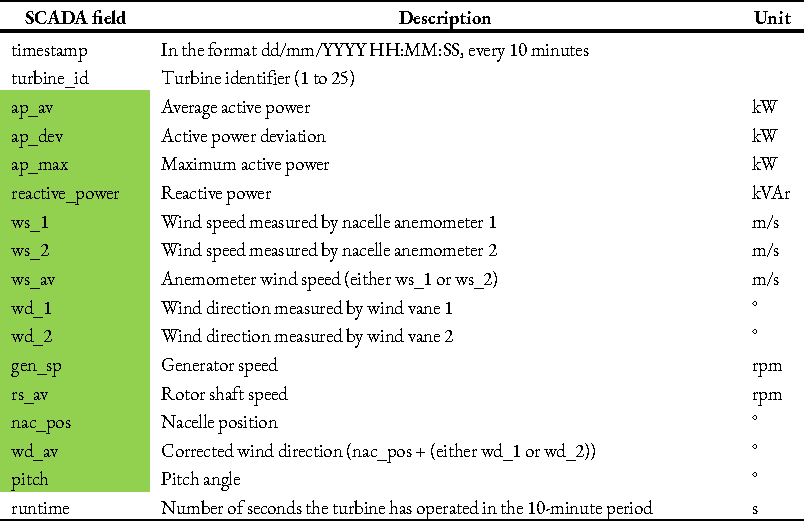
\includegraphics{t1.pdf}
    \caption{\label{t1}Summary of SCADA fields for the SCADA data used in this project. The fields include timestamps with a resolution of 10 minutes, average active power, wind speed, pitch and runtime. The fields that contain measurements averaged over the 10-minute period are highlighted in green. These measurements can be used as features in machine learning as they are turbine properties.}
\end{table}

The downtime data consists of fields summarised in Table~\ref{t2}. Each row of downtime data consists of the start and end timestamps of the downtime event, downtime categories, workorders and alarms. Downtime categories, which are turbine, environmental, grid, infrastructure and availability categories, describes the turbine's condition or cause of downtime when the maintenance work was undertaken. Each condition within each downtime category is represented by a unique identifier in the dataset. A separate spreadsheet accompanying the dataset list what each identifier stands for. All quantities in the downtime data, except the alarms, are supervised (i.e., the data recordings are input and monitored by maintenance professionals).

\begin{table}
    \centering
    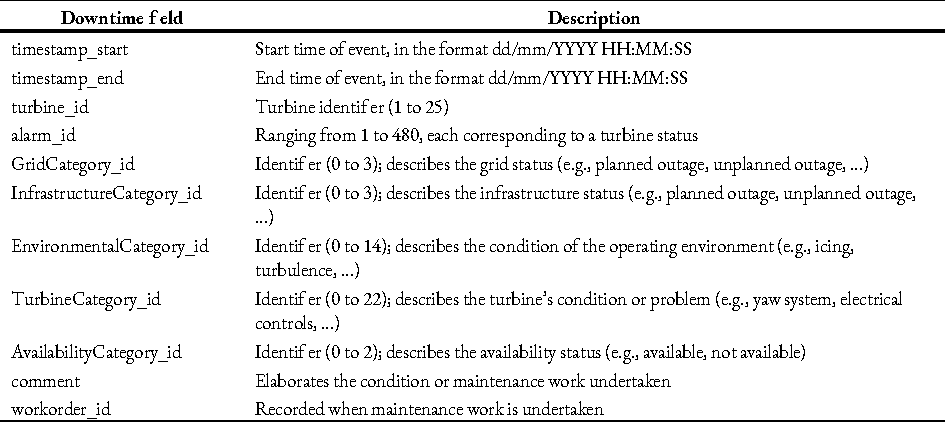
\includegraphics{t2.pdf}
    \caption{\label{t2}Summary of fields for the downtime data used in this project. The fields include start and end timestamps for the downtime event, downtime categories, workorders and alarms.}
\end{table}

Each row of SCADA data requires a class which describes the state of the turbine. The chosen classes are `normal' for normal behaviour, and `faulty' to signify a fault. As the aim is to predict faults in advance, a category of classes, called `before fault' will also be used. To automate the labelling process, the SCADA data can be merged with the downtime data, which has turbine categories, listed in Table~\ref{t3}, that can be used to label faults. Some of these turbine categories, such as `OK' and `scheduled maintenance', do not indicate a fault in the turbine, and `other' does not specify the condition. Therefore, only the turbine categories which indicate faults, highlighted in green, are used to class the SCADA data. Prior to merging the two datasets, the downtime data is restructured such that it has the same 10-minute resolution as the SCADA data. The SCADA data was also found to have missing rows of data. Empty data rows with only the timestamp corresponding to the missing rows were added to rectify this. Once they are merged, 14 separate labels, or columns, are added for each specific fault, which will allow for the different faults to be distinguished. The rows with a fault category are classed as `faulty' in the corresponding column.

\begin{table}
    \centering
    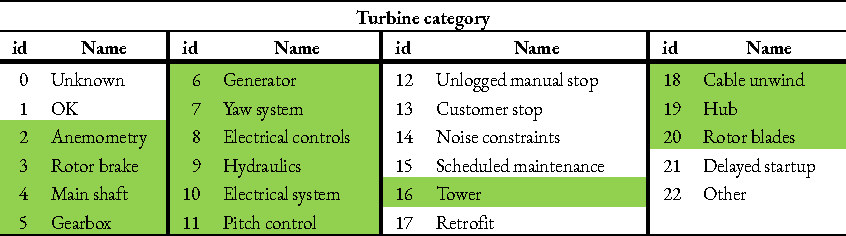
\includegraphics{t3.pdf}
    \caption{\label{t3}List of turbine categories in the wind farm downtime data. The categories used as the different faults for labelling are highlighted in green. The others do not indicate a fault.}
\end{table}

To summarise the machine learning terminology used, features refer to SCADA fields which are turbine properties, labels refer to turbine categories or type of fault, and classes refer to the state of the turbine (e.g., `normal' or `faulty') for each row of data at each label. The features and labels will be fit to a classifier for training as arrays X of size [rows, 10] and Y of size [rows, 14] respectively, where rows refer to the number of rows in the training data.

To predict faults for each label, rows with timestamps up to 48 hours in advance of a `faulty' row are classed at 6-hour intervals (i.e., up to X hours before a fault, where X = 6, 12, \dots, 48). The reasons for having classes of 6-hour intervals for fault detection rather than a single class is to allow action to be taken appropriate to the time before fault. For example, if it is predicted that the wind turbine could have a fault in six hours or less, it could be switched off to prevent further damage from occurring. 48 hours is enough time for maintenance professionals to travel to site and carry out inspection, and decide on what action to take. Depending on the nature of the site, this value can be modified (i.e., for an offshore wind farm which operates in harsh environments, it is more likely to take a longer time to travel to the site and complete works relative to an onshore wind farm).

% Power curves are used to help with labelling as they are easier to visualise due to the distinct power curve shape which represents wind turbine performance. Figure 2 .1(a) shows the labelled power curve for turbine 2 with turbine category 16, where many curtailment and anomalous points are classed as `normal'. These should be removed as they deviate from the typical power curve shape which indicates normal behaviour. To filter out the curtailment, the pitch angle should be within a typical threshold for `normal' data points between 10\,\% and 90\,\% power. Data points with power below 10\,\% and above 90\,\% are not included, pitch angles often deviate from 0\,\textdegree in these operating regions, due to the control of the turbine. To find this threshold, the most frequent pitch angles are quantified, with 0\,\textdegree being the most frequent. Filtering out points with a pitch angle exceeding 0\,\textdegree, however, distorts the power curve shape, removing a large portion of points in the region where it transitions to rated power. To prevent this, pitch angles between 0\,\textdegree and 10\,\textdegree were tested as the threshold, with 3.5\,\textdegree producing the best result (see Appendix A1. for full results). The effects of applying this filter can be seen in Figure  2 .1(b), which still has anomalous points below 10\,\% and above 90\,\% power. To remove these, additional filters are applied to `normal' data points at operating wind speeds, including removing zero power, and turbine categories and other downtime categories that are not faults or `OK', and runtime of less than 600 s. There is a vertical line of data points at zero wind speed which is removed using a power threshold of 100 kW before the cut-in speed of 3 m/s. It is necessary to use this threshold because the nacelle anemometer wind speed, which is used to plot these power curves, is not an accurate measure of the wind speed incident on the turbine blades, and removing all data points exceeding 0 kW power before cut-in results in a distorted power curve shape (see Appendix A2.). The threshold is based on the minimum power before cut-in that does not distort the power curve shape for all 25 turbines. The result of applying these filters is shown in Figure  2 .1(c).

% \begin{figure}
%     \centering
%     \begin{subfigure}[t]{0.5\textwidth}
%         \centering
%         \includegraphics[height=1.2in]{a}
%         \caption{Lorem ipsum}
%     \end{subfigure}%
%     ~
%     \begin{subfigure}[t]{0.5\textwidth}
%         \centering
%         \includegraphics[height=1.2in]{b}
%         \caption{Lorem ipsum, lorem ipsum,Lorem ipsum, lorem ipsum,Lorem ipsum}
%     \end{subfigure}
%     \caption{Caption place holder}
% \end{figure}

% <!-- figure goes here -->

% Rows of data with missing features and labels are removed, as all fields must be complete for classification. Instead of deleting the rows of data corresponding to the data points removed from the `normal' class, they are classed as `curtailment'. This is because the data points removed are specific to one label, which means they are not necessarily classed as `normal' for other labels, and it is important for the classifier to learn the different states of the turbine for each fault. To summarise, the classes used are `normal', `faulty', `curtailment' and `up to X hours before fault' (where X = 6, 12, \dots, 48). 



% Figure 2.1: Changes to the power curve of turbine 2 with the fault points corresponding to when the turbine category is 16 (`tower') through the two stages of filtering out anomalous and curtailment points labelled as `normal'. The original power curve is shown in (a). The first stage involves a filter based on a pitch angle threshold, which produces (b). The second stage involves several additional filters to produce the final power curve (c).

\section{Classification}

% Since there are numerous classifiers offered in scikit-learn, this is narrowed down to a manageable number for comparison. As explained above, each row of SCADA data, or sample, has multiple labels that require classification into multiple classes, which makes this a multiclass-multilabel problem. There are presently three classification algorithms on scikit-learn with the ability to classify multiclass-multilabel problems, namely decision trees (DT), random forests (RF) and k nearest neighbours (kNN). [CITATION sci168 \l 1033 ] Therefore, only these three classifiers are evaluated in this project.

% DT is a simple technique which uses a tree structure to ask a series of questions with conditions to split data with different attributes. [ CITATION Yon10 \l 1033 ] While DT only uses a single tree, RF constructs multiple trees which perform the classification to determine the class, with the majority class among all trees being selected, therefore producing a classifier better than DT.  [CITATION Leo17 \l 1033 ] Meanwhile, for kNN, the class of a test sample is determined by comparing the sample to a number of closest neighbouring training samples. [CITATION Oli12 \m Jak17 \l 1033 ] Each classifier consists of hyperparameters which can be optimised for specific data for better performance. An example is the number of neighbours, or k, for kNN, which is a user-defined positive integer.

% The data used in this project is highly imbalanced (i.e., the number of samples for `normal' class is in thousands for each turbine, while the `faulty' and `X hours before fault' classes only range from tens to a few hundreds). This can cause the classifier to be biased towards the majority class and perform poorly on minority classes. [CITATION sci162 \l 1033 ] The effect of balancing data is investigated by doing classification with and without class balancing. The balancing is done by oversampling all classes using the imbalanced-learn library's random over sampler [CITATION GLe161 \l 1033 ] prior to feeding the training data into the classifiers. Oversampling is done instead of random sampling, because it will not reduce the amount of data, which causes loss of information. This oversampling does not support multilabel classification (i.e., it only accepts array Y of size [rows, 1]), therefore separate estimators will be used for each fault. This means that for each turbine, using the imbalanced multilabel approach would only require one estimator which trains on all labels simultaneously, while using the balanced dataset approach requires separate estimators for each of the 14 faults which cannot run in parallel. Oversampling also results in increased number of samples, which in turn increases the time taken to train a classifier.

% To increase reliability of the results, a five-fold cross-validation is performed. Traditionally, the dataset would be split into five sets for a five-fold cross-validation, with four being used for training the classifier and the remaining one for testing. In each fold, the training and testing set combinations would be different. The performance is measured for each fold and averaged to give the final score. Since SCADA data is a time series, it is likely that the data points collected over time have some form of correlation, which must be considered when being analysed. [ CITATION Nat13 \l 1033 ] Therefore, this makes the traditional cross-validation unsuitable, as it does not take the order of the data into account. The data is divided using scikit-learn's time series split, which includes the preceding set of data in successive splits. [CITATION sci167 \l 1033 ] Figure  2 .2 illustrates the difference between traditional and time series split cross-validations. Optimising the hyperparameters of a classifier based on the average performance over cross-validation folds prevents the training data from overfitting to the classifier, which happens when the classifier performs well during training but poorly on testing or unseen future data. [CITATION Jea16 \m Lia16 \l 1033 ]

% <!-- figure goes here -->

% Figure 2.2: Illustration of traditional cross-validation and time series split cross-validation, both five-folds. In time series split, shown on the right, the order of data is taken into account.

% Prior to cross-validation, the features are normalised [ CITATION sci171 \l 1033 ] to a scale of 0 to 1. This is important as the features used in classification have vastly different scales. For example, the turbine data sheet gives generator operating speeds of between 740 rpm and 1,300 rpm, while the wind speeds recorded by the anemometers range from 0 m/s up to 34 m/s. Normalisation preserves the characteristics and distribution of the features and prevents potential problems that could arise due to features with drastically different scales when classification is done. [CITATION Mic17 \l 1033 ]

% A number of performance metrics are available on scikit-learn to assess classifier performance. [ CITATION sci17 \l 1033 ] Precision is the ratio of true positives,  to the sum of  and false positives, , as shown in Equation ( 2 .1). Equation ( 2 .2) describes recall, which is the ratio of  to the sum of  and . [ CITATION And15 \l 1033 ] F1 score, shown in Equation ( 2 .3), is the harmonic average of precision and recall. [ CITATION Ric17 \l 1033 ] The reason for not using accuracy is because it does not distinguish between  and . [ CITATION Ric17 \l 1033  \m SAS17] The metrics compute the scores for each class individually which are averaged, taking into account the support, which is the number of data points belonging to each class in the test set, to produce the final weighted score. The higher the scores, the better the performance of the classifier.  and  both have costs. [ CITATION Ric17 \l 1033 ] However, it is unknown at the moment which is more important for this wind farm. Therefore, the optimisations will use the F1 score as the main performance metric. As these metrics are not supported for multilabel classification, the execution is performed in a loop for each label. This means for each turbine, each cross-validation fold will output one score for each label, producing 70 scores in total. These can then be averaged for each turbine or fault to produce a final score.

% <!-- equations go here -->

% The classification is carried out as a process. The first step is to use cross-validation to optimise some initial hyperparameters of the classifiers, namely criterion for DT and RF, and weights for kNN. The criterion is either `entropy' or the default `gini', while weights is either `distance' or the default `uniform'. The classification is done once using imbalanced data as it is, and once using balanced training data. After evaluating whether balancing the data improves the classifier's performance, further hyperparameters can be tuned.
